\documentclass{book}
% comment out the following line if you want to latex the whole book:
%\includeonly{ch9}
  % preamble

\usepackage{verbatim}\usepackage{epsf}

\setlength{\textwidth}{5.2in}            % default seems to be around 4.8 inch,
\addtolength{\evensidemargin}{-0.2in}    % so we can devide the extra 0.4 inch
\addtolength{\oddsidemargin}{-0.2in}     % equally over left and right margin

\setlength{\parindent}{2.5em}
\setlength{\parskip}{1.2 ex plus0.2ex minus 0.1ex}
\renewcommand{\baselinestretch}{1.05}
\renewcommand{\floatpagefraction}{1.0}
\renewcommand{\topfraction}{1.0}

\begin{document}
  \frontmatter
\makebox[3.5in][s]{}\verb=Time-stamp: <2002-04-12 13:22:51 piet>=
%
% nice latex feature: you can specify which files you want to include in your
% next output, by listing only those files as arguments to \includeonly{} 
% above on the third line (I had to put this comment here, since the emacs
% time stamp is only recognized in the first eight lines).
% NOTE: if you want to print out the whole book, simply comment out the line
% starting with \includeonly above.
%
% It is a good idea to write this top level file out, each time a change has
% been made, in order to get the correct time stamp to appear on the title
% page.  Even if you print out only one chapter, still the title page will
% appear, so that the time stamp will be include (otherwise the time stamp
% would appear uselessly on a separate white page, before the chapter).
%
    \def\half{{\ifmmode{{1 \over 2}}\else{${1 \over 2}$}\fi}}
\def\dhalf{{\textstyle {1 \over 2}}}
\def\threehalf{{\ifmmode{{3 \over 2}}\else{${3 \over 2}$}\fi}}
\def\dthreehalf{{\textstyle {3 \over 2}}}
\def\dfivehalf{{\textstyle {5 \over 2}}}
\def\dfivethree{{\textstyle {5 \over 3}}}
\def\bx{{\bf x}}
\def\br{{\bf r}}
\def\bv{{\bf v}}
\def\ba{{\bf a}}
\def\bj{{\bf j}}
\def\bs{{\bf s}}
\def\bc{{\bf c}}
\def\bp{{\bf p}}
\def\bk{{\bf k}}
\def\badot{{\bf \dot a}}
\def\batwo{{{\bf  a}^{(2)}}}
\def\bathree{{{\bf  a}^{(3)}}}
\def\bR{{\bf R}}
\def\bV{{\bf V}}
           % input, not include, since all files need the \def{}
    % title page

\thispagestyle{empty}                 % suppresses page numbering of first page

\begin{latexonly}

\begin{center}


\hbox{}

\bigskip\bigskip


{\lggggb Moving Stars Around}

\bigskip


\bigskip\bigskip


{\lggb A Preliminary Version}


\medskip


{\lggb of what will expand into}


\medskip

{\lggb Volumes 1,2,3}

\medskip

{\lggb of the series}

\bigskip\bigskip

{\lgggb The Art of Computational Science}

\bigskip\bigskip

\end{center}

\end{latexonly}


\begin{htmlonly}


\begin{center}


\hbox{}

\bigskip\bigskip


{\huge \bf Moving Stars Around}

\medskip


{\LARGE A Preliminary Version}



{\LARGE of what will expand into}


\medskip



{\LARGE Volumes 1,2,3}

\medskip



{\LARGE of the series}


\bigskip


{\huge \bf The Art of Computational Science}



\bigskip


\end{center}
\end{htmlonly}

 \begin{latexonly}
 \begin{center}
 \leavevmode
 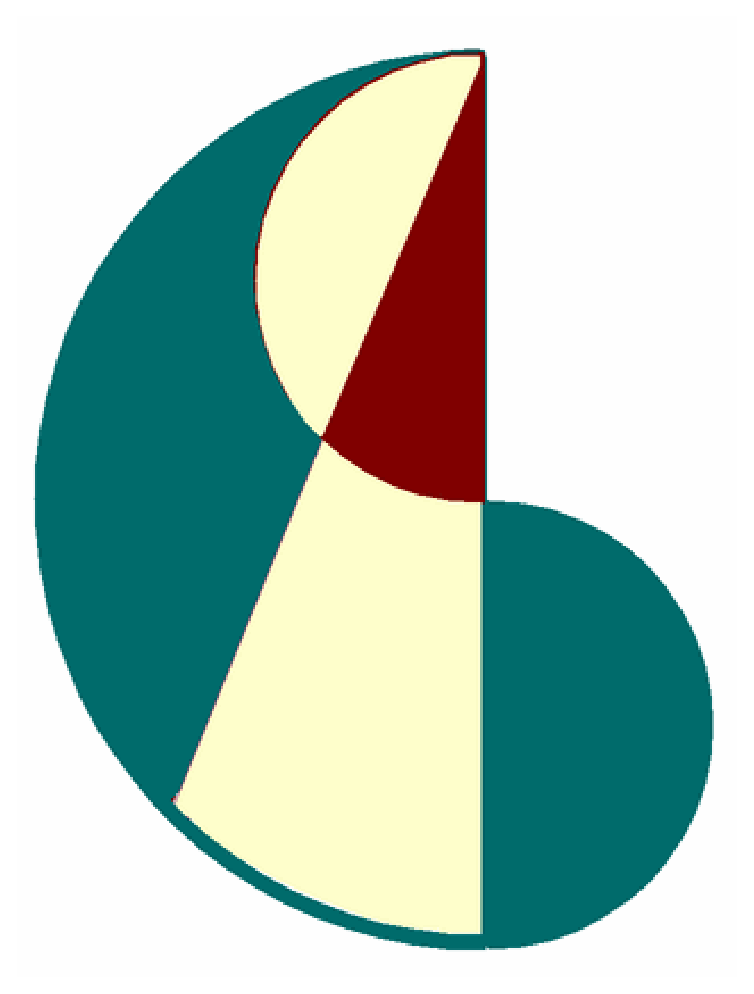
\includegraphics[width=4cm]{acstitle.eps}
 \end{center}
 \end{latexonly}


\begin{htmlonly}
\begin{center}
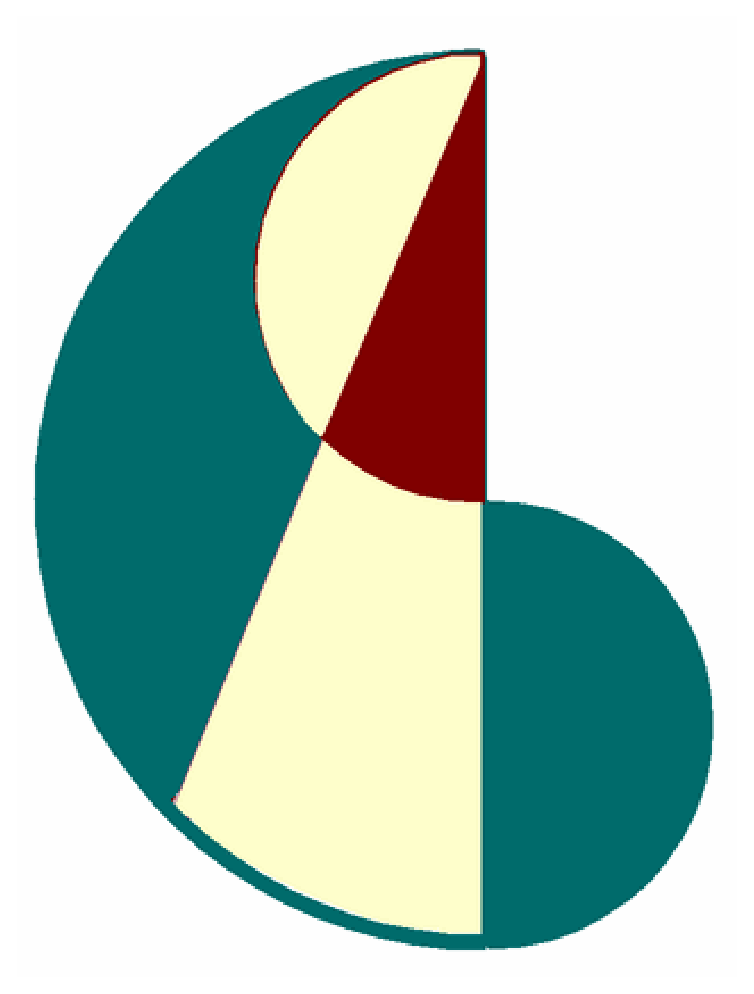
\includegraphics[width=3cm]{acstitle.eps}
\end{center}
\end{htmlonly}

\bigskip\bigskip\bigskip


\begin{center}
% lggr -> Large
% lr -> large
\begin{tabular}{llllllll}
& {\LARGE Piet Hut} & {\LARGE \&} & & & & & {\LARGE Jun Makino}\\
&  & & & & & & \\
& {\large Institute for Advanced Study} & & & & & &
  {\large Univ. of Tokyo, \ Dept. of Astronomy}\\
& {\large 1 Einstein Drive} & & & & & & {\large 7-3-1 Hongo, Bunkyo-ku}\\
& {\large Princeton, NJ 08540} & & & & & & {\large Tokyo 113-0033}\\
& {\large U.S.A.} & & & & & & {\large JAPAN}\\
& {\large piet@ias.edu} & & & & & & {\large makino@astron.s.u-tokyo.ac.jp}\\
\end{tabular}

\bigskip\bigskip\bigskip\bigskip

\end{center}
         % input, in order to let the time stamp appear
%
% uncomment the following three lines, if you want to print two pages
% on one, using e.g. "psnup -2 v1.ps > v1_2.ps".  Normally the next three
% lines should be commented out, but in that case psnup will print the right
% (left) pages on the left (right) side.
%
%\newpage
%\thispagestyle{empty}
%\mbox{}
%
    \newpage           % blank page, to force preface to start on a right hand page
\thispagestyle{empty}      % suppresses page numbering of the blank second page
\mbox{}                    % dummy content; otherwise \newpage has no effect
\newpage                   % on to third page, to start the preface
\pagenumbering{roman}      % with a roman numbering system, starting here at i

%%\chapter{Preface} %% this replace the four lines below, but at the
                    %% cost (currently) of two extra pages

\addcontentsline{toc}{chapter}{Preface}

\begin{center}
{\lgb Preface}
\end{center}

The {\it Pure Gravity} book series, of which this is the second volume,
\dots\dots\dots

%\bigskip
%\bigskip
%{\it Acknowledgments:}
%xxx
%We thank xxx, xxx and xxx for valuable
%discussions.  This work is supported in part by the Research for the
%Future Program of Japan Society for the Promotion of Science
%(JSPS-RFTP97P01102).

\tableofcontents

\listoffigures


  \mainmatter
      \chapter{The Universe in a Computer}

\section{Gravity}

Gravity is the weakest of all fundamental forces in physics, far
weaker than electromagnetism or the so-called weak and strong
interactions between subatomic particles.  However, the other three
forces lose out in the competition with gravity over long distances.
The weak and strong interactions both have an intrinsically short
range.  Electromagnetism, while being long-range like gravity, suffers
from a cancellation of attraction and repulsion in bulk matter, since
there tend to be as almost exactly as many positive as negative
charges in any sizable piece of matter.  In contrast, gravitational
interactions between particles are always attractive.  Therefore, the
larger a piece of matter is, the more gravitational force it exerts on
its surroundings.

This dominance of gravity at long distances makes the job of
modeling a chunk of the Universe easier.  To a first approximation, it
is often a good idea to neglect the other forces, and to model the
objects as if they were interacting only through gravity.  In many
cases, we can also neglect the intrinsic dimensions of the objects,
treating each object as a point in space with a given mass.  All this
greatly simplifies the mathematical treatment of a system, by leaving
out most of the physics and chemistry that would be needed in a more
accurate treatment.

This book is the first in a series of books titled {\it Pure Gravity}, to
indicate that we are making this approximation of treating objects as
gravitating masses and nothing more.  The objects we will be studying
are stars, and the environment we will focus on are dense stellar
systems, where the stars are so close together that they will
occasional collide and in general have frequent interesting and
complex interactions.  In a later series, {\it Applied Gravity}, we will
look at the internal physics of those stars: how they evolve under the
influence of nuclear reactions in their centers, how they may die in
cosmic explosions, and what happens to their remnant cores.  We will
especially study how interactions between stars of all types can change
their evolutionary behavior through two-body, three-body, and more
complex interactions, leading to an intricate `star cluster ecology'.

This first book, {\it Writing an N-Body Code}, lays the groundwork for
modeling a system of stars.  We start absolutely from scratch, with a
most simple code of less than a page long.  In many small steps we
then improve that code, pointing out the many pitfalls along the way,
on the level of programming as well as astrophysical understanding.
We introduce helpful code development facilities and give many hints as
to how to balance simplicity, efficiency, clarity, and modularity of
the code.  Our intention is to introduce the topic from square one,
and then to work our way up to a robust set of codes with which one
can do actual research.  In later volumes in this series, we will
continue to develop these codes, adding many useful diagnostic tools,
and integrating those in a full production-level software environment.

\section{Galactic Suburbia}

The sun is a star like any other among the hundred billion or so stars
in our galaxy.  It is unremarkable in its properties.  Its mass is in
the mid range of what is normal for stars: there are others more than
ten times more massive, and there are also stars more ten times less
massive, but the vast majority of stars have a mass within a factor
ten of that of the sun.  Our home star is also unremarkable in its
location, at a distance of some thirty thousand light years from the
center of the galaxy.  Again, the number of stars closer to the center
and further away from the center are comparable.  Our closest neighbor,
Proxima Centauri, lies at a distance of a bit more than four light years.

This distance is typical for separations between stars in our neck of
the woods.  A light year is ten million times larger than the diameter
of the sun (a million km, or three light seconds).  In a scale model,
if we would represent each star as a cherry, an inch across, the
separation between the stars would be many hundreds of miles.  It is
clear from these numbers that collisions between stars in the solar
neighborhood must be very rare.  Although the stars follow random
orbits without any traffic control, they present such tiny targets
that we have to wait very long indeed in order to witness two of them
crashing into each other.  A quick estimate tells us that the sun has
a chance of hitting another star of less than $10^{-18}$ per year.  In
other words, we would have to wait at least $10^{18}$ years to have an
appreciable chance to witness such a collision.  Given that the sun is
less than five billion years old, it is no surprise that it does not
show any signs of a past collision: the chance that that would have
happened was less than one in a hundred million.  Life in our galactic
suburbs is really quite safe for a star.

There are other places in our galaxy that are far more crowded, and
consequently are a lot more dangerous to venture into.  We will have
a brief look at four types of crowded neighborhoods.

\section{Globular Clusters}

\begin{figure}[ht]
\centering
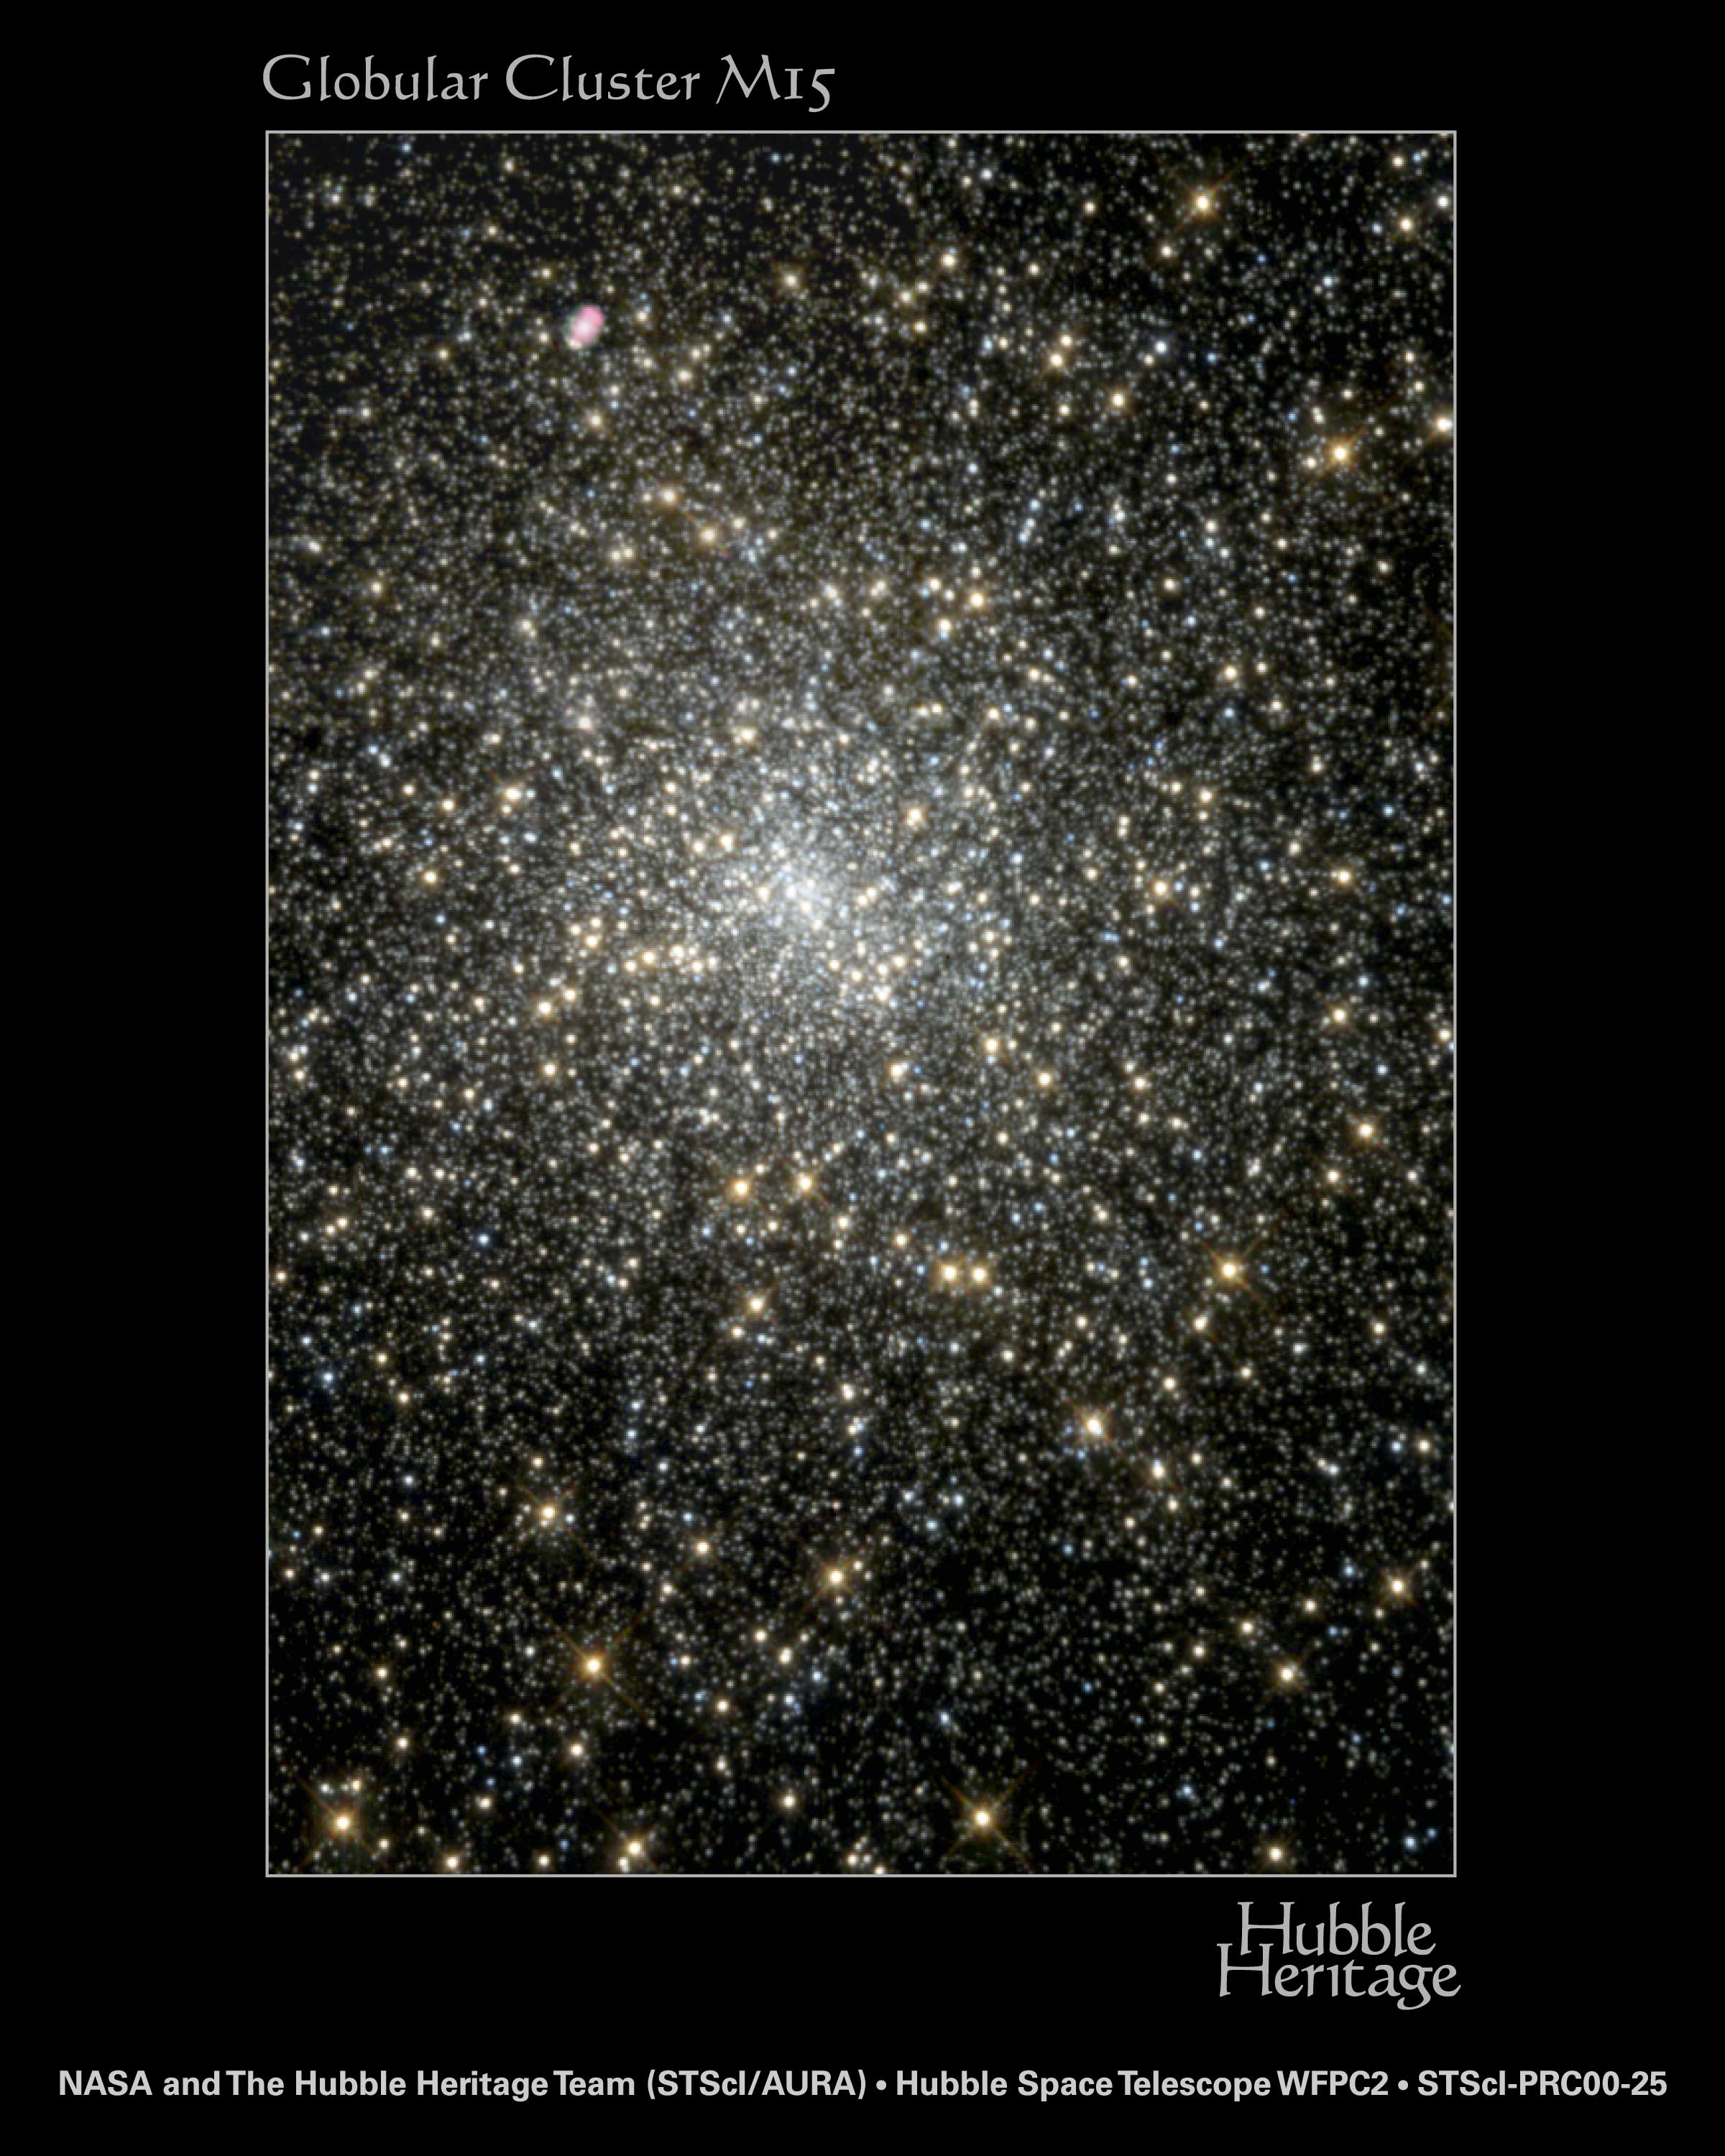
\includegraphics[width=4.5in]{chap1/m15.eps}
\caption[A snapshot of the globular cluster M15]
{A snapshot of the globular cluster M15, taken with the Hubble Space
Telescope.}
\label{fig:m15}
\end{figure}
%%  From: http://oposite.stsci.edu/pubinfo/PR/2000/25/content/0025y.jpg

In Fig. \ref{fig:m15} we see a picture of the globular cluster M15,
taken with the Hubble Space Telescope.  This cluster contains roughly
a million stars.  In the central region typical distances between
neighboring stars are only a few hundredth of a light year, more than
a hundred times smaller than those in the solar neighborhood.  This
implies a stellar density that is more than a million times larger
than that near the sun.  Since the typical relative velocities of
stars in M15 are comparable to that of the sun and its neighbors, a
few tens of km/sec, collision times scale with the density, leading to
a central time between collisions of less than $10^{12}$ years.  With
globular clusters having an age of more than $10^{10}$ years, a typical
star near the center already has a chance of more than a percent to
have undergone a collision in the past.  

In fact, the chances are much higher than this rough estimate indicates.
One reason is the stars spend some part of their life time in a much
more extended state.  A star like the sun increases its diameter by
more than a factor of one hundred toward the end of its life, when
they become a red giant.  By presenting a much larger target to other
stars, they increase their chance for a collision during this stage
(even though this increase is partly offset by the fact that the red
giant stage lasts shorter than the so-called main-sequence life time
of a star, during which they have a normal appearance and diameter).
The other reason is that many stars are part of a double star system,
a type of dynamic spider web that can catch a third star, or another
double star, into a temporary three- or four-body dance.  Once engaged
in such a dance, the local stellar crowding is enormously enhanced,
and the chance for collisions is greatly increased. 

A detailed analysis of all these factors predicts that a significant
fraction of stars in the core of a dense globular cluster such as M15
has already undergone at least one collision in its life time.  This
analysis, however, is quiet complex.  To study all of the important
channels through which collisions may occur, we have to analyze
encounters between a great variety of single and double stars, and
occasional bound triples and larger bound multiples of stars.  Since
each star in a bound subsystem can be a normal main-sequence star, a
red giant, a white dwarf, a neutron star or even a black hole, as well
as an exotic collision product itself, the combinatorial richness of
flavors of double stars and triples is enormous.  If we want to pick a
particular double star, we not only have to choose a star type for
each of its members, but in addition we have to specify the mass of
each star, and the parameters of its orbit, such as the semimajor axis
(a measure for the typical separation of the two stars) as well as the
orbital eccentricity.

The goal of our book series is to develop the software tools to make
it possible to simulate an entire star cluster like M15, and to
analyze the resulting behavior both locally and globally.

\clearpage  % to let the m15 picture be inserted not further than here

\section{Galactic Nuclei}

In Fig. \ref{fig:gc} we see an image of the very center of our galaxy.
This picture is taken with the Northern branch of the two Gemini
telescopes, which is located in Hawaii on top of the mountain Mauna Kea.

\begin{figure}[ht]
\centering
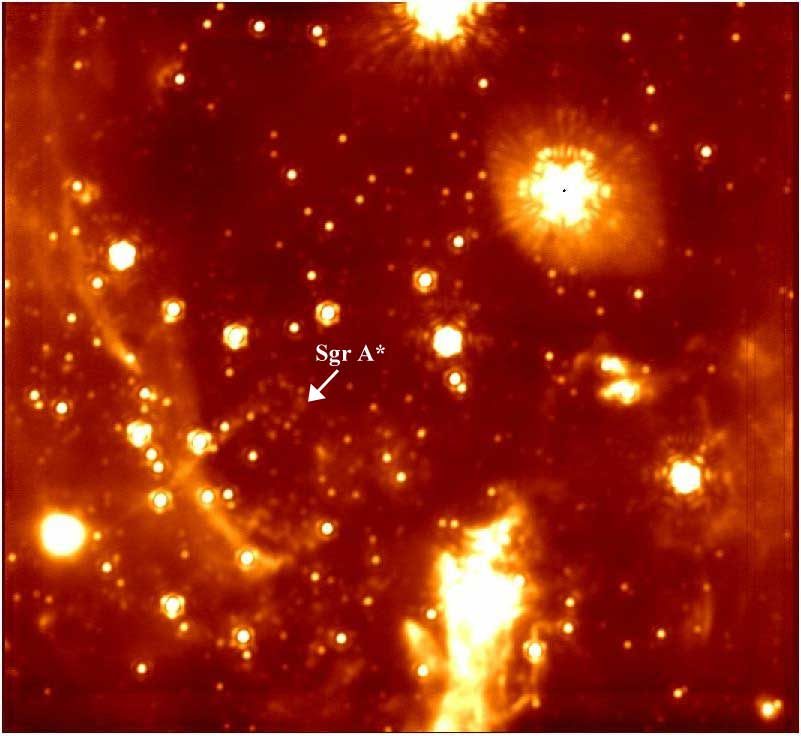
\includegraphics[width=4.5in]{chap1/gc.eps}
\caption[An image of the central region of our galaxy]
{An image of the central region of our galaxy, taken with the Gemini
North telescope.  The center is located on the right just above the
bottom edge of the image.}
\label{fig:gc}
\end{figure}
%% From: http://www.gemini.edu/gallery/observing/gc\_color.jpg

In the very center of our galaxy, a black hole resides with a mass
a few million times larger than the mass of our sun.  Although the
black hole itself is invisible, we can infer its presence by its
strong gravitational field, which in turn is reflected in the speed
with which stars pass near the black hole.  In normal visible light it
is impossible to get a glimpse of the galactic center, because of the
obscuring gas clouds that are positioned between us and the center.
Infrared light, however, can penetrate deeper in dusty regions.
Fig. \ref{fig:gc} is a false-color image, reconstructed from
observations in different infrared wavelength bands.

In the central few light years near the black hole, the total mass of
stars is comparable to the mass of the hole.  This region is also
called the galactic nucleus.  Here the stellar density is at least as
large as that in the center of the densest globular clusters.  However,
due to the strong attraction of the black hole, the stars zip around at
much higher velocities.  Whereas a typical star in the core of M15 has
a speed of a few tens of km/sec, stars near the black hole in the
center of our galaxy move with speeds exceeding a 1000 km/sec.  As a
consequence, the frequency of stellar collisions is strongly enhanced.

Modeling the detailed behavior of stars in this region remains a great
challenge, partly because of the complicated environmental features.
A globular cluster forms a theorist's dream of a laboratory, with its
absence of gas and dust and starforming regions.  All we find there
are stars that can be modeled well as point particles unless they come
close and collide, after which we can apply the point particle
approximation once again.  In contrast, there are giant molecular
clouds containing enormous amounts of gas and dust right close up to
the galactic center.  In these clouds, new stars are formed, some of
which will soon afterwards end their life in brilliant supernova
explosions, while spewing much of their debris back into the
interstellar medium.  Such complications are not present in globular
clusters, where supernovae no longer occur since the member stars are
too old and small to become a supernova.

Most other galaxies also harbor a massive black hole in their nuclei.
Some of those have a mass of hundreds of millions of solar masses, or
in extreme cases even more than a billion times the mass of the sun.
The holy grail of the study of dense stellar systems is to perform and
analyze accurate simulations of the complex ecology of stars and gas
in the environment of such enormous holes in space.  Much of the
research on globular clusters can be seen as providing the initial
steps toward a detailed modeling of galactic nuclei.

\section{Star Forming Regions}

\begin{figure}[ht]
\centering
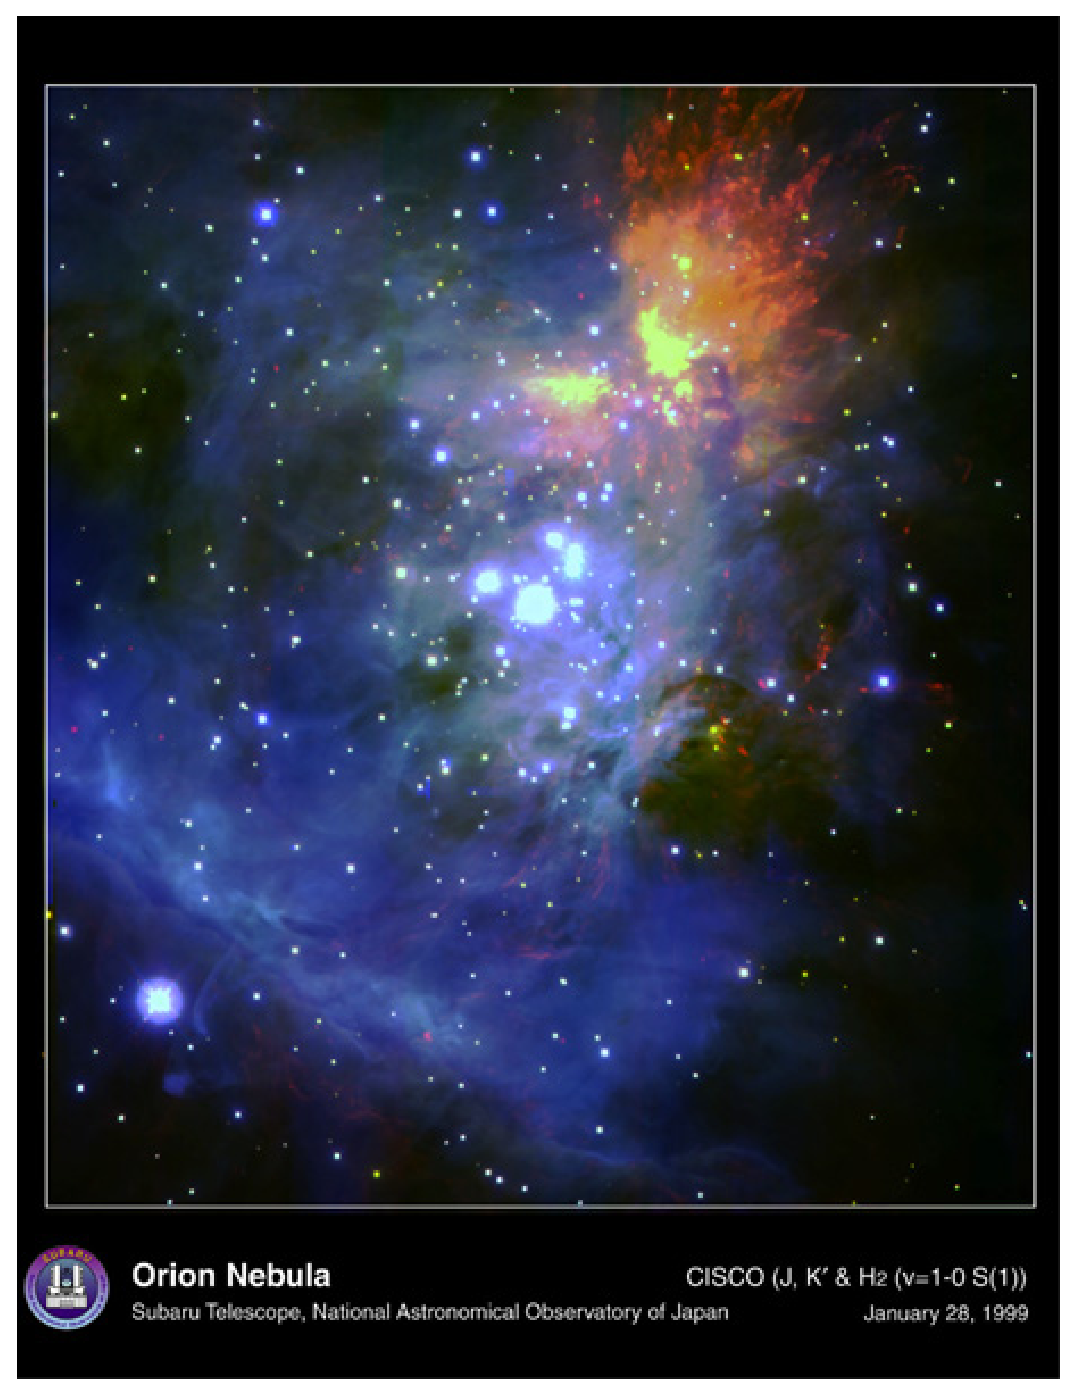
\includegraphics[width=3in]{chap1/orion.eps}
\caption[The Orion Nebula]
{The Orion Nebula, as seen by the Subaru telescope.}
\label{fig:orion}
\end{figure}
%%  From: http://www.subaru.naoj.org/Science/press\_release/9901/Orion.jpg

There are many other places in the galactic disk where the density of
stars is high enough to make collisions likely, at least temporarily.
These are the sites where stars are born.  Fig. \ref{fig:orion} taken
by the Japanese Subaru telescope in Hawaii shows the Orion Nebula,
also known as M42, at a distance of 1500 light years from the sun.
This picture, too, is taking in infrared light in order to penetrate
the dusty regions surrounding the young stars.  The four brightest
stars in the center, collectively known as the Trapezium, form the
most massive stars of a larger conglomeration of stars, all recently
formed from the gas and dust that still surrounds them.

In order to study collisions in these star forming regions, we can no
longer treat the stars are point masses.  Many of the collisions take
place while the stars are still in the process of forming.  While a
protostar is still in the process of contracting from the gas cloud
in which it was born, it presents a larger target for collisions with
other stars.  In addition, a single contracting gas cloud may fission,
giving rise to more than one star at the same time.  In this way, the
correlated appearance of protostars is even more likely to lead to
subsequent collisions.

The proper way to model these processes is to combine gas dynamics and
stellar dynamics.  Much progress has been made recently in this area.
One way to use stellar dynamics in an approximate fashion is to begin
with the output of the gas dynamics codes, which present the positions
and velocities of a group of newly formed stars, and then to follow
and analyze the motions of those stars, including their collisions.

\section{Open Clusters}

Although stars are formed in groups, these groups typically do not
stay together for very long.  Perturbations from other stars and gas
clouds in their vicinity are often enough to break up the fragile
gravitational hold they initial have over each other.  Some of the
more massive groups of newly formed stars, however, are sufficiently
tightly bound to survive their environmental harassment.  They form
the so-called open clusters, where there name indicates that they have
central densities that are typically less than what we see in globular
clusters.

\begin{figure}[ht]
\centering
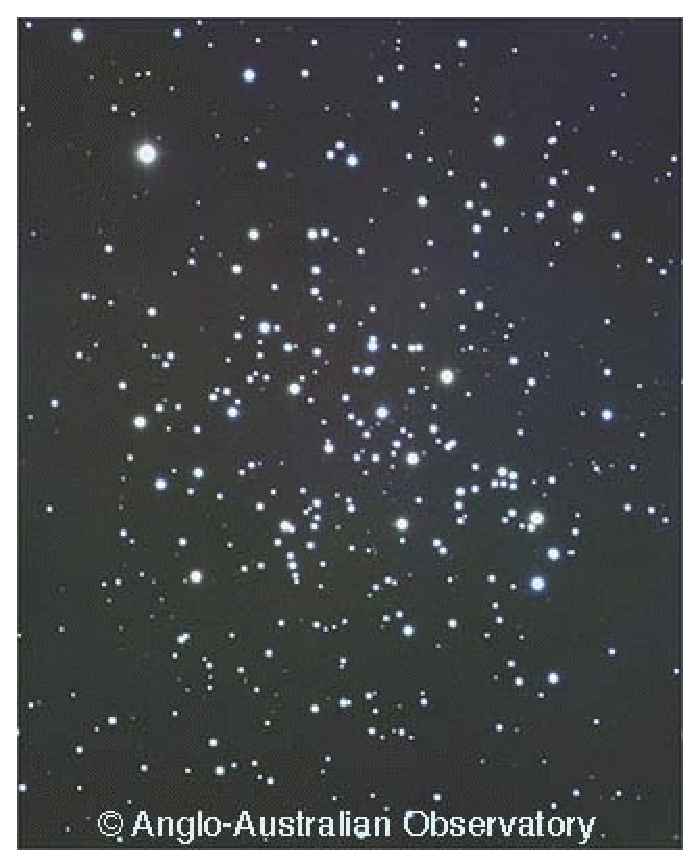
\includegraphics[width=2.5in]{chap1/m67.ps}
\caption[The open star cluster M67]
{The open star cluster M67, in a picture taken by the Anglo-Australian
Observatory.}
\label{fig:m67}
\end{figure}
%%  From: http://www.seds.org/messier/Pics/More/m67aat.jpg

Fig. \ref{fig:m67} shows one of the richest and densest open clusters,
M67, as observed by the Anglo-Australian Observatory.  Since this
cluster is old enough to have lost its gas and dust, all stars are
visible at normal optical wavelengths, at which this image is taken.
In the central regions of this cluster, there are indications that
some of the stars have undergone close encounters or even collisions.
Consequently, this star cluster qualifies as a dense stellar system.

Open clusters typically have fewer members than globular clusters.
Also, they are younger.  Both facts makes it easier to simulate open
clusters than globular clusters.  On the other hand, the densest
globular clusters show a higher frequency and a far richer variety of
stellar collisions, making them a more interesting laboratory.  In
that sense, a dynamical simulation of an open cluster can be seen as
providing preparatory steps toward the modeling of globular clusters,
just as a study of the latter forms a stepping stone toward the
investigation of galactic nuclei.

\section{Writing your own star cluster simulator}

Astronomers have almost half a century of experience in writing
computer codes to simulate dense stellar systems.  The first published
results date back to 1960, and it was in the subsequent decade that it
became clear just how tricky it was to simulate a group of interacting
stars.  The task seems so easy: just integrate Newton's equations of
motion for each star, under the influence of the gravitational pairwise
interactions of all other stars.  Indeed, it is straightforward to
write a simple code to do so, as we will see below.  And as long as
all stars remain fairly well separated from each other, even a simple
code will do a reasonably good job.

In practice, though, even a small group of stars will spontaneously
form one or more double stars.  This was discovered experimentally in
the early sixties.  One way to understand this result, after the fact,
is from an energetic point of view.  When a double star, or binary as they
are generally called, is formed, energy is released.  Since the two stars
in a binary are bound, the potential energy is larger than the kinetic
energy, and the total energy is negative.  When three stars come together
randomly, there is a chance that two of the three are left in a bound
state, while the third one escapes, carrying the excess energy.  Left
by itself, a stellar system will exploit this energy liberation
mechanism by spontaneously forming binaries.

As soon as even one binary appears, a simple code with constant time
steps will either crash or resort to a very slow and inefficient crawl.
The changes in the relative configuration of the two stars occur so
frequent that they can be easily missed.  If they are modeled correctly,
by choosing a tiny time step, the rest of the system will be forced to
slow down, while spending a large and unnecessary amount of computer
time on all the other stars that don't need such fine resolution.  By
the end of the sixties, these problems were overcome by the development
of codes that employed individual time steps.  Stars with close
neighbors were stepped forward in time more frequently than stars at
large, and in this way the computational power was brought to where it
was most needed.

This modification in itself brought gravitational $N$-body codes already
well outside the range of systems that are normally discussed in text
books on numerical integration methods.  The internal book keeping
needed to write a correct and efficient code with individual time
steps is surprisingly large, given the simplicity of the task:
integrate the effect of pairwise attractive inverse square forces.
But this was only a first step toward the development of modern $N$-body
codes.  The presence of tight binaries produced much more of an obstacle,
and throughout the seventies a variety of clever mechanisms were developed
in order to deal with them efficiently.

For one thing, there are problems with round-off.  Two stars in a tight
orbit around each other have almost the same position vector, as seen
from the center of a star cluster, where we normally anchor the global
coordinate system.  And yet it is the separation between the stars
that determines their mutual forces.  When we compute the separation
by subtracting two almost identical spatial vectors, we are asking for
(numerical) trouble.  The solution is to introduce a local coordinate
system whenever two or more stars undergo a close interaction.  This
does away with the round-off problem, but it introduces a host of
administrative complexities, in order to make sure that any arbitrary
configuration of stars is locally presented correctly -- and that the
right thing happens when two or more of such local coordinate patches
encounter each other.  This may not happen often, but one occurrence
in a long run is enough to crash the system if no precautions have
been taken for such a situation to happen.

We can continue the list of tricks that have been invented to allow
every larger and denser systems to be modeled correctly.  Numerical
problems with the singularity in the two-body system have been
overcome by mapping two or more interacting stars from the
three-dimensional Kepler problem to a four-dimensional harmonic
oscillator.  The total force on particles has been split into
different contributions, the first from a near zone of relatively
close neighbors and the second from a far zone of all other particles,
with each partial force being governed with different integration time
steps.  Tree codes have been used to group the contributions of a
number of more and more distant zones together in ever larger chunks,
for efficiency.  Triple stars have received their own special treatment,
especially the marginally stable triples that are sometimes long-lived, 
but continuously changed their inner state due to internal perturbations.
The list goes on.

In this first book, we will introduce a modern integrator, the Hermite
scheme, developed in the 1990s, together with a variable time step
integration scheme, where all stars share a common time step at any
given time.  In subsequent volumes in the series, we will introduce
the other refinements mentioned above.  Our emphasis will be on a
complete explanation of all the steps involved, together with a
discussion of the motivation for those steps.  In the last few
chapters, we will embark on a research project featuring stellar
collisions, in a simple gravity-only approximation.

    \part{Object Oriented $N$-Body Codes}
      \chapter{Regularization}


      \chapter{Setting Up and Analyzing Gravitational Scattering Experiments}


    \part{Mini Gravitylab}
      \chapter{A Story-Telling Mechanism}


      \chapter{Automatization of Laboratory Experiments}


    \part{Astrophysical Applications}
      \chapter{Exploring $N = 3$ with a Hermite Algorithm}

Having seen the dramatic improvement that came from switching from the
forward Euler algorithm to the leapfrog, the obvious next step was to
go to yet higher order algorithms.  A quick look in a few books of
numerical methods showed our friends that there was a bewildering
choice of third- and fourth-order methods to choose from.  Alice then
mentioned that her thesis advisor had pointed her to an elegant and
natural generalization of the leapfrog algorithm, by the name of the
Hermite scheme.

\section{A Surprisingly Simple Hermite Scheme}

The most symmetric Hermite version, and the one closest resembling the
leapfrog is this one:

\def\half{{\textstyle\frac{1}{2}}}
\def\quarter{{\textstyle\frac{1}{4}}}
\def\one#1{{\textstyle\frac{1}{#1}}}
\def\three#1{{\textstyle\frac{3}{#1}}}
\def\seven#1{{\textstyle\frac{7}{#1}}}

\begin{eqnarray}
\br_{i+1} & = & \br_i + \half(\bv_i + \bv_{i+1}) dt +
                \one{12}(\ba_i - \ba_{i+1})(dt)^2
                \label{hermite-step1} \\
\bv_{i+1} & = & \bv_i + \half(\ba_i + \ba_{i+1}) dt +
                \one{12}(\bj_i - \bj_{i+1})(dt)^2
                \label{hermite-step2}
\end{eqnarray}

Here $\bj = d\ba/dt$ is the {\it jerk}, the time derivative of the
acceleration, and therefore the third time derivative of position:

\begin{equation}
\bj = \frac{d^3}{dt^3} \br
\end{equation}

The term `jerk' has crept into the literature relatively recently,
probably originally as a pun.  If a car or train changes acceleration
relatively quickly you experience not a smoothly accelerating or
decelerating motion, but instead a rather `jerky' one.

The jerk can be computed through straightforward differentiation of
Newton's gravitational equations, Eq. \ref{newton}:

\begin{equation}
\bj_i =  G \sum_{j=1 \atop j \neq i}^N \,M_j \left[
\frac{\bv_{ji}}{r_{ji}^3} - 3 \frac{(\br_{ji}\cdot\bv_{ji})\br_{ji}}{r_{ji}^5}
\right]\label{newton-jerk}
\end{equation}

\noindent
where $\bv_{ji} = \bv_j - \bv_i$.

As an aside, note that the jerk has one very convenient property.
Although the expression above looks quite a bit more complicated than
Newton's original equations, they can still be evaluated through one
pass over the whole $N$-body system.  This is no longer true for
higher derivatives.  For example, we can obtain the fourth derivative
of the position of particle $i$ (the {\it snap}, see next section) by
differentiating Eq. \ref{newton-jerk}:

\begin{eqnarray}
\frac{d^4}{dt^4}\br_i = G \sum_{j=1 \atop j \neq i}^N \,M_j \Bigg[ &\,&
\!\!\!\!\!\!\!\!\!\! \frac{\ba_{ji}}{r_{ji}^3}
-6 \frac{(\br_{ji}\cdot\bv_{ji})}{r_{ji}^5}\bv_{ji} \nonumber \\
 &\,& \!\!\!\!\!\!\!\! + \left\{ -3\frac{v_{ji}^2}{r_{ji}^5}
-3 \frac{(\br_{ji}\cdot\ba_{ji})}{r_{ji}^5}
+15 \frac{(\br_{ji}\cdot\bv_{ji})^2}{r_{ji}^7} \right\} \br_{ji} \,\,\Bigg]
\label{newton-snap}
\end{eqnarray}

\noindent
where $\ba_{ji} = \ba_j - \ba_i$, and this is the expression that
thickens the plot.  Unlike the $\br_{ji}$ and $\bv_{ji}$ expressions,
that are given by the initial conditions, $\ba_{ji}$ has to be
calculated from the positions and velocities.  However, this
calculation does not only involve the pairwise attraction of particle
$j$ on particle $i$, but in fact all pairwise attractions of all
particles on each other!  This follows immediately when we write out
what the shorthand implies:

\begin{equation}
\ba_{ji} = \ba_j - \ba_i = G \sum_{k=1 \atop k \neq j}^N
\frac{M_k}{r_{kj}^3} \,\br_{kj} -  G \sum_{k=1 \atop k \neq i}^N
\frac{M_k}{r_{ki}^3} \,\br_{ki}
\end{equation}

\noindent
When we substitute this back into Eq. \ref{newton-snap}, we see that
we have to do a double pass over the $N$-body system, summing over
both indices $k$ and $j$ in order to compute a single fourth derivative
for the position of particle $i$.  

\section{Comparison with the Leapfrog}

When we look at Eqs. \ref{hermite-step1}, \ref{hermite-step2}, we see
some familiar features.  Neglecting the higher-order term for the
moment, we recognize the leapfrog: the new position is effectively
determined by the mid-point velocity $v_{i+1/2}$, here approximated as
the average between the two adjacent values $v_{i}$ and $v_{i+1}$.
Similarly, the new velocity is effectively determined by the mid-point
acceleration.

In fact, the analogy can be made more precise.  Recalling the leapfrog,
as written centered on integer times, Eqs. \ref{leapfrog-step1},
\ref{leapfrog-step2}:

\begin{eqnarray}
\br_{i+1} & = & \br_i + \bv_{i} dt + \ba_{i} (dt)^2/2 \label{leapfrog-step1a}\\
\bv_{i+1} & = & \bv_i + (\ba_i + \ba_{i+1})dt / 2 \label{leapfrog-step2a}
\end{eqnarray}

\noindent
we can transform these back into a pseudo-leap form, without using
half-integer times explicitly, by rewriting the first equation as:

\begin{eqnarray}
\br_{i+1} & = & \br_i + \half(\bv_{i} + \bv_{i+1}) dt
                      + \half(\bv_{i} - \bv_{i+1}) dt
                      + \half\ba_{i} (dt)^2 \nonumber \\
	  & = & \br_i + \half(\bv_{i} + \bv_{i+1}) dt
                      + \quarter(-\ba_i-\ba_{i+1})(dt)^2
                      + \half\ba_{i}(dt)^2 \nonumber \\
	  & = & \br_i + \half(\bv_{i} + \bv_{i+1}) dt
                      + \quarter(\ba_i-\ba_{i+1})(dt)^2 \nonumber \\
	  & = & \br_i + \half(\bv_{i} + \bv_{i+1}) dt - \quarter\bj_i (dt)^3
                                                      \label{leapfrog-trick}
\end{eqnarray}

In the second line, we have simply rearranged terms.  In the third
line, we have used \ref{leapfrog-step2a}, and in the fourth line we
have used the definition of $\bj$, while neglecting higher order terms
in $dt$.

The next step is to remember that the leapfrog is a second-order scheme.
The errors per step are $\propto(dt^3)$, and therefore it does not
matter whether or not we include the last term $-\bj_i (dt)^3/4$ into
our leapfrog version: this term is lost in the noise, and is not going
to improve the accuracy on second-level order.  Therefore, we may
equally well leave it out.  Doing so transforms Eqs. \ref{leapfrog-step1a},
\ref{leapfrog-step2a} into:

\begin{eqnarray}
\br_{i+1} & = & \br_i + \half(\bv_i + \bv_{i+1})dt \label{leapfrog-step1b} \\
\bv_{i+1} & = & \bv_i + \half(\ba_i + \ba_{i+1})dt \label{leapfrog-step2b}
\end{eqnarray}

Here we see explicitly that our good old leapfrog is equivalent, up to
its second-order accuracy, with the leading terms $\propto (dt)$ of
the Hermite algorithm, Eqs. \ref{hermite-step1}, \ref{hermite-step2}.
It is a curiosity of the leapfrog that at first sight it resembles a
first-order scheme, since the second-order terms are hidden in the
`leapy' way of using average quantities.  Yet, as we have seen, the
leapfrog is fully second-order.

In a very similar way, the Hermite scheme is fourth-order, even though
it resembles a second-order scheme.  For details we refer to the
literature, but it is interesting to see in a heuristic way why this
is so.

\section{Snap, Crackle, and Pop}

First a word about terminology.  We will need to introduce a few extra
derivatives of the position.  It would be fun to give them names with
a reasonable `feel' to them, just like with jerk.  What type of motion
feels even more restless than jerking motion?  A sudden snap comes to
mind.  A what changes its state more sudden than a snap --- how about
a crackle?  And for those familiar with American rice crispies culture,
a pop cannot be far away, and indeed, if something pops it really
changes high derivatives of positions in a substantial way!  We are
not making these names up: we have seen them used a few times before,
although the precise source is likely to be lost in (recent) history.
So here they are:

\begin{equation}
\bs = \frac{d^4}{dt^4} \br \qquad ; \qquad
\bc = \frac{d^5}{dt^5} \br \qquad ; \qquad
\bp = \frac{d^6}{dt^6} \br
\end{equation}

\noindent
{\it snap}, {\it crackle}, and {\it pop}, respectively.

We are now in a position to write the Taylor series for the four
quantities that appear in Eqs. \ref{hermite-step1}, \ref{hermite-step2},
up to crackle:

\begin{eqnarray}
\br_{i+1} & = & \br_i + \bv_i dt + \half\ba_{i}(dt)^2 + \one{6}\bj_{i}(dt)^3
                      + \one{24}\bs_{i}(dt)^4 + \one{120}\bc_{i}(dt)^5
                                                           \label{taylor-r} \\
\bv_{i+1} & = & \bv_i + \ba_i dt + \half\bj_{i}(dt)^2 + \one{6}\bs_{i}(dt)^3
                      + \one{24}\bc_{i}(dt)^4              \label{taylor-v} \\
\ba_{i+1} & = & \ba_i + \bj_i dt + \half\bs_{i}(dt)^2 + \one{6}\bc_{i}(dt)^3
                                                           \label{taylor-a} \\
\bj_{i+1} & = & \bj_i + \bs_i dt + \half\bc_{i}(dt)^2      \label{taylor-j}
\end{eqnarray}

\noindent
We can now eliminate snap and crackle at time $t_i$, expressing them
in terms of the acceleration and jerk at times $t_i$ and $t_{i+1}$,
using Eqs. \ref{taylor-a}, \ref{taylor-j}.  We find:

\begin{eqnarray}
\bs_i &=& 6(\ba_{i+1} -\ba_{i})(dt)^{-2} -2(\bj_{i+1} +2\bj_{i})(dt)^{-1} \\
\bc_i &=& -12(\ba_{i+1} -\ba_{i})(dt)^{-3} +6(\bj_{i+1} +\bj_{i})(dt)^{-2}
\end{eqnarray}

\noindent
Substituting both expressions in Eq. \ref{taylor-v} we directly find:

\begin{equation}
\bv_{i+1} = \bv_i + \half(\ba_i + \ba_{i+1}) dt +
                \one{12}(\bj_i - \bj_{i+1})(dt)^2 \label{hermite-step2a}
\end{equation}

\noindent
Indeed, we have recovered Eq. \ref{hermite-step2}, and thereby
explained the mysterious factor $\one{12}$ in the last term.

Let us complete our mission, by making the same derivation for 
the position vector, Eq. \ref{hermite-step1}, in the Hermite scheme.
Using again the snap and crackle expressions derived above, we find:

\begin{equation}
\br_{i+1} = \br_i + \bv_i dt + (\seven{20}\ba_i + \three{20}\ba_{i+1})(dt)^2
            + (\one{20}\bj_i - \one{30}\bj_{i+1})(dt)^3
\end{equation}

\noindent
Using the same trick we employed in Eq. \ref{leapfrog-trick} to factor
out the velocity terms, and using Eq. \ref{hermite-step2a}, we can
rewrite the above expression as:

\begin{equation}
\br_{i+1} = \br_i + \half(\bv_i + \bv_{i+1}) dt
            + \one{10}(\ba_i - \ba_{i+1})(dt)^2
            + \one{120}(\bj_i + \bj_{i+1})(dt)^3
\end{equation}

\noindent
While this result still looks quite different from Eq. \ref{hermite-step1},
we claim that it is identical up to fourth-order in $dt$, which is all we
need.  Our final step thus parallels the discussion following
Eq. \ref{leapfrog-trick} for the leapfrog, where we had to show how
terms up to second-order were identical.

First we rewrite the above equation in terms of quantities defined at $t=i$:

\begin{eqnarray}
\br_{i+1} = \br_i + \half(\bv_i + \bv_{i+1}) dt 
             & + & \one{10}\ba_i(dt)^2 - \one{10}(\ba_i + \bj_i dt +
              \half\bs_i (dt)^2)(dt)^2                           \nonumber \\
          & + & \one{120}\bj_i(dt)^3 + \one{120}(\bj_i + \bs_i dt)(dt)^3
                                                                 \nonumber \\
          = \br_i + \half(\bv_i + \bv_{i+1}) dt 
          & - & \one{12}\bj_i (dt)^3 - \one{24} \bs_i (dt)^4
\end{eqnarray}

\noindent
Here we have left out terms containing $\bc_i$, since they would be
proportional to at least $(dt^5)$ and only contribute to the error noise.
We can similarly write out the last term of Eq. \ref{hermite-step1}:

\begin{eqnarray}
\one{12}(\ba_i - \ba_{i+1})(dt)^2  & = & 
              \one{12}\left(\ba_i(dt)^2 - \one{12}(\ba_i + \bj_i dt +
              \half\bs_i (dt)^2)\right)(dt)^2                     \nonumber \\
             & = & - \one{12}\bj_i (dt)^3 - \one{24} \bs_i (dt)^4
\end{eqnarray}

\noindent
This proves the desired result:

\begin{equation}
\br_{i+1} = \br_i + \half(\bv_i + \bv_{i+1}) dt +
                \one{12}(\ba_i - \ba_{i+1})(dt)^2
\end{equation}

\section{Implementing Hermite}

Let us return to Alice, Bob, and Carol, who are about to implement the
Hermite scheme.  Since Bob was most eager to test out this new
algorithm, he got his turn behind the computer.

\abc

\bob
Let's give this new Hermite scheme a stress test.  I'll take {\st
leapfrog2a.C}, the one with the off-set in initial velocity of
$10^{-4}$, call it {\st hermite1a.C} for now, and simply substitute
the leapfrog equations \ref{leapfrog-step1}, \ref{leapfrog-step2} by
the Hermite equations \ref{hermite-step1}, \ref{hermite-step2}.

\carol
Why not call the code {\st hermite1.C}?

\bob
Even though the update seems almost trivial, I don't have the audacity
to believe we'll get everything right the first time around.  When it
all works, we will rename the code to {\st hermite1.C}.  So here is
the new version:

\cba

\code{hermite1a.C}{chap6/hermite1a.C}

\abc

\alice
Ah, I see now that you were wise giving the code an preliminary name.
Notice where you have added the jerk calculation.  You replaced

\begin{small}
\begin{verbatim}
            for (int k = 0; k < 3; k++){
                a[i][k] += m * rji[k] / r3;
                a[j][k] -= m * rji[k] / r3;
            }
\end{verbatim}
\end{small}

\noindent
by:

\begin{small}
\begin{verbatim}
            for (int k = 0; k < 3; k++){
                a[i][k] += m * rji[k] / r3;
                a[j][k] -= m * rji[k] / r3;
                jk[i][k] += m * (vji[k] - 3 * rv * rji[k]) / r3;
                jk[j][k] -= m * (vji[k] - 3 * rv * rji[k]) / r3;
            }
\end{verbatim}
\end{small}

\noindent
in addition to some extra changes, such as introducing and calculating
the variable {\st vji[]} for the relative velocities for particles $i$
and $j$.  All of this is fine, as far as I can see.  The statements are
correctly written and reflect the Hermite, but there is one problem.
In the last two lines above you use the relative velocities $vij[]$,
but at this point in the program they have not been assigned yet.

\bob
Ah, you are right.  That happens just a few lines below, with this
`clever' trick of using the magnitude of the centrifugal acceleration
to determine the magnitude of the velocities.  Thanks!  Okay, so I'll
make another version, {\st hermite1b.C}, which has two initial loops,
one for the accelerations, followed by the assignment of velocities,
and then followed by the second loop which computes the jerks.

\carol
Maybe we can just run the program using our friend {\st /dev/null} to
see how the energy behaves, before start making pictures.  I'm really
curious to see whether we have now reached fourth-order accuracy.

\bob
Easy to test:

\cba

\begin{small}
\begin{verbatim}
|gravity> g++ -o hermite1b hermite1b.C
|gravity> hermite1b > /dev/null
Please provide a value for the time step
0.01
and for the duration of the run
100
Initial total energy E_in = -0.866025
Final total energy E_out = -0.975389
absolute energy error: E_out - E_in = -0.109364
relative energy error: (E_out - E_in) / E_in = 0.126282
|gravity> !!
hermite1b > /dev/null
Please provide a value for the time step
0.001
and for the duration of the run
100
Initial total energy E_in = -0.866025
Final total energy E_out = -0.866586
absolute energy error: E_out - E_in = -0.000560173
relative energy error: (E_out - E_in) / E_in = 0.000646832
|gravity> !!
hermite1b > /dev/null
Please provide a value for the time step
0.0001
and for the duration of the run
100
Initial total energy E_in = -0.866025
Final total energy E_out = -0.866026
absolute energy error: E_out - E_in = -5.52839e-07
relative energy error: (E_out - E_in) / E_in = 6.38364e-07
|gravity> !!
hermite1b > /dev/null
Please provide a value for the time step
0.00001
and for the duration of the run
100
Initial total energy E_in = -0.866025
Final total energy E_out = -0.866025
absolute energy error: E_out - E_in = -5.53711e-10
relative energy error: (E_out - E_in) / E_in = 6.39371e-10
|gravity> 
\end{verbatim}
\end{small}

\abc

\carol
What is this?  We seem to have constructed a third-order algorithm!

\alice
Hmmm.  It seems that way.  Each refinement of a factor ten in step
size gives a reduction of the error of a factor 1000.  But this was
not supposed to happen

\bob
This is strange indeed.  Look, at the end, there they are, the real
Hermite expressions, what can be wrong with such simple statements??

\begin{small}
\begin{verbatim}
        for (int i = 0; i < n; i++){
            for (int k = 0; k < 3; k++){
                r[i][k] = old_r[i][k] + (old_v[i][k] + v[i][k])*dt/2
                                      + (old_a[i][k] - a[i][k])*dt*dt/12;
                v[i][k] = old_v[i][k] + (old_a[i][k] + a[i][k])*dt/2
                                      + (old_j[i][k] - jk[i][k])*dt*dt/12;
            }
        }
\end{verbatim}
\end{small}

\carol
Yes, they are just what we derived before, as Eqs. \ref{hermite-step1},
\ref{hermite-step2}.

\alice
Could we have made a similar mistake as we did just before, when the
expressions were absolutely correct, but the order of execution was wrong?

\bob
Well \dots hmmm \dots aha, of course, you are right!  Look, that is
exactly the problem.  In the first line, where the position is updated,
we indicate that we are using both the old velocity values and the new
velocity values.  However, the new ones have not been computed yet ---
that happens only on the next line!  And the solution is obvious:
fortunately, the second line updating the velocity does not have this
problem, since it uses only accelerations and jerks, all of which have
already been computed, both for the old and the new values.  So we can
simply swap the lines, and this should now work:

\begin{small}
\begin{verbatim}
        for (int i = 0; i < n; i++){
            for (int k = 0; k < 3; k++){
                v[i][k] = old_v[i][k] + (old_a[i][k] + a[i][k])*dt/2
                                      + (old_j[i][k] - jk[i][k])*dt*dt/12;
                r[i][k] = old_r[i][k] + (old_v[i][k] + v[i][k])*dt/2
                                      + (old_a[i][k] - a[i][k])*dt*dt/12;
            }
        }
\end{verbatim}
\end{small}

\section{Testing the Hermite: Three Stars on a Circle}

\bob
Now I'm ready to be brave and call the code {\st hermite1.C}.  Rather
than listing the whole output, let me use the {\st diff} program,
which only lists those lines that are different.

\cba

\begin{small}
\begin{verbatim}
|gravity> diff hermite1a.C hermite1.C
2c2
< // hermite1a.C
---
> // hermite1.C
30c30
<             a[i][k] = jk[i][k] = 0.0;
---
>             a[i][k] = 0.0;
33,34c33,34
<             double rji[3], vji[3];
<             for (int k = 0; k < 3; k++){
---
>             double rji[3];
>             for (int k = 0; k < 3; k++)
36,37d35
<                 vji[k] = v[j][k] - v[i][k];
<             }
42,45d39
<             double rv = 0;
<             for (int k = 0; k < 3; k++)
<                 rv += rji[k] * vji[k];
<             rv /= r2;
49,50d42
<                 jk[i][k] += m * (vji[k] - 3 * rv * rji[k]) / r3;
<                 jk[j][k] -= m * (vji[k] - 3 * rv * rji[k]) / r3;
64a57,81
>     for (int i = 0; i < n; i++)
>         for (int k = 0; k < 3; k++)
>             jk[i][k] = 0.0;
>     for (int i = 0; i < n; i++){
>         for (int j = i+1; j < n; j++){
>             double rji[3], vji[3];
>             for (int k = 0; k < 3; k++){
>                 rji[k] = r[j][k] - r[i][k];
>                 vji[k] = v[j][k] - v[i][k];
>             }
>             double r2 = 0;
>             for (int k = 0; k < 3; k++)
>                 r2 += rji[k] * rji[k];
>             double r3 = r2 * sqrt(r2);
>             double rv = 0;
>             for (int k = 0; k < 3; k++)
>                 rv += rji[k] * vji[k];
>             rv /= r2;
>             for (int k = 0; k < 3; k++){
>                 jk[i][k] += m * (vji[k] - 3 * rv * rji[k]) / r3;
>                 jk[j][k] -= m * (vji[k] - 3 * rv * rji[k]) / r3;
>             }
>         }
>     }
> 
127,128d143
<                 r[i][k] = old_r[i][k] + (old_v[i][k] + v[i][k])*dt/2
<                                       + (old_a[i][k] - a[i][k])*dt*dt/12;
130a146,147
>                 r[i][k] = old_r[i][k] + (old_v[i][k] + v[i][k])*dt/2
>                                       + (old_a[i][k] - a[i][k])*dt*dt/12;
|gravity>
\end{verbatim}
\end{small}

\abc

\carol
Yes, that is much clearer than listing the whole source code again.
I can see how the main difference has been the move of the jerk
calculation from the earlier part, where it was entangled with the
acceleration calculation, to a separate block listed nearly at the
end.  At the very end, of course, there is the indication that we have
swapped the order of the calculations of the positions and the velocities.
The {\st diff} program arbitrarily took the velocity calculation as a
identical standard in each file, with respect to which the shift in
order of the position calculation was noted.

\alice
Soon we should start to clean up our codes, splitting them in
functions at least, and probably also in different files.  That way we
don't have to rely on {\st diff} to read our own programs, since we
can then take natural chunks at a time, in the form of functions.  But
first let's see what will happen to our figure 8 orbits.

\bob
Here are the results.  Hmm, not a very good energy conservation, if
you ask me.

\cba

\begin{small}
\begin{verbatim}
|gravity> g++ -o hermite1 hermite1.C
|gravity> hermite1 > hermite1_0.01_100.out
Please provide a value for the time step
0.01
and for the duration of the run
100
Initial total energy E_in = -0.866025
Final total energy E_out = -1.08608
absolute energy error: E_out - E_in = -0.220054
relative energy error: (E_out - E_in) / E_in = 0.254096
|gravity>
\end{verbatim}
\end{small}

\abc

\carol
Indeed.  The leapfrog did far better at this stage.  We got a relative
energy error of less than $10^{-3}$, and here we are faced with a relative
energy error of a quarter!

\alice
That is not so strange, actually.  A higher-order algorithm computes
higher-order derivatives, and therefore can be extra sensitive to
close encounters or other situations in which changes happen quite
suddenly.  Let's look at the picture, and then move on, refining our
step size.

\cba

\begin{figure}[htb]
\begin{center}
\epsfxsize = 2.5in
\epsffile{chap6/hermite1_0.01_100.ps}
\caption[Three stars on a circle, Hermite, $dv_{init}=0.0001$, $dt = 0.01$,
$t_{end} = 100$]
{The first Hermite attempt to integrate the orbits of three stars
starting off on a circle with an initial velocity perturbation of 
$dv_{init}=0.0001$, time step $dt = 0.01$ and a total duration of
$t_{end} = 100$}
\label{fig:hermite1-0.01-100}
\end{center}
\end{figure}

\begin{small}
\begin{verbatim}
|gravity> hermite1 > hermite1_0.001_100.out
Please provide a value for the time step
0.001
and for the duration of the run
100
Initial total energy E_in = -0.866025
Final total energy E_out = -0.866026
absolute energy error: E_out - E_in = -9.19142e-07
relative energy error: (E_out - E_in) / E_in = 1.06133e-06
|gravity>
\end{verbatim}
\end{small}

\begin{figure}[htb]
\begin{center}
\epsfxsize = 2.5in
\epsffile{chap6/hermite1_0.001_100.ps}
\caption[Three stars on a circle, Hermite, $dv_{init}=0.0001$, $dt = 0.001$,
$t_{end} = 100$]
{The second Hermite attempt to integrate the orbits of three stars
starting off on a circle with an initial velocity perturbation of 
$dv_{init}=0.0001$, time step $dt = 0.001$ and a total duration of
$t_{end} = 100$}
\label{fig:hermite1-0.001-100}
\end{center}
\end{figure}

\abc

\carol
Ah, much better!  Amazing.

\bob
An improvement of more than a factor 100,000 in accuracy!

\carol
And look at the picture.  I cannot see any difference between Fig. 
\ref{fig:hermite1-0.001-100} and the last picture in the series that
we did with the leapfrog, Fig. \ref{fig:leap2a-0.00001-100}!

\alice
Let's take another refinement step, to see whether we can determine
the asymptotic behavior of the error growth.  Clearly, our first
attempt was not reliable, so we need at least a third try.

\cba

\begin{small}
\begin{verbatim}
|gravity> hermite1 > hermite1_0.0001_100.out
Please provide a value for the time step
0.0001
and for the duration of the run
100
Initial total energy E_in = -0.866025
Final total energy E_out = -0.866025
absolute energy error: E_out - E_in = -8.49854e-12
relative energy error: (E_out - E_in) / E_in = 9.81326e-12
|gravity>
\end{verbatim}
\end{small}

\begin{figure}[htb]
\begin{center}
\epsfxsize = 2.5in
\epsffile{chap6/hermite1_0.0001_100.ps}
\caption[Three stars on a circle, Hermite, $dv_{init}=0.0001$, $dt = 0.0001$,
$t_{end} = 100$]
{The third Hermite attempt to integrate the orbits of three stars
starting off on a circle with an initial velocity perturbation of 
$dv_{init}=0.0001$, time step $dt = 0.0001$ and a total duration of
$t_{end} = 100$}
\label{fig:hermite1-0.0001-100}
\end{center}
\end{figure}

\abc

\carol
Okay, Bob, you can call this code {\st hermite1.C}, it seems to do its job.

\bob
But it does its job too well.  Another five magnitudes of error improvement.
Now it behaves like a fifth order code.

\alice
This seems to happen sometimes.  A $k$th-order scheme is guaranteed
only to have errors that grow not faster than $k$th order.  However,
it is possible for them to grow less fast.  For example, it could be
that the particular orbits we are studying just happen to have some
properties that lead to cancellations in some of the orders.

\carol
Is there any reason to believe that we do not have a generic system here?

\alice
Don't forget that we are studying a rather unstable system, in which
it is quite likely that we will have at least one close encounter
between two or three particles.  So far, we have been sailing blindly,
hoping that the step size we give the integrator is small enough to
prevent near-collisions or other forms of strange behavior during
close encounters.  Soon we'll have to do better, though.  It is not
too hard to predict close encounters when they are about to happen,
and to adapt the integration step size automatically.  Only with such
safety precautions does it make sense to rigorously measure the
performance of the algorithm, whether it is the leapfrog or the
Hermite.  Without such precautions, even slight changes could show a
different behavior.  For example, cleaning up the code by initializing
the velocities directly, instead of using the centrifugal trick, is
likely to give slightly different initial conditions.  I would not
be surprised if such a change would give us yet another scaling of the
errors, if we repeat the above measurements.

\bob
Okay, I guess we are ready to do quite a bit of cleaning up in our code.
It is getting a bit too spaghetti-like for my taste already.  Let's do
that next time.  We can improve readability and functionality at the
same time, while we go along.

\carol
For now though, I feel that the Hermite should be our tool of choice.
It sure seems to converge must faster.  How about doing a timing test?

\bob
Good idea.  Let's do it with the figure-8 orbits though.  There at
least we do not have any close encounters, so Alice's warnings may
carry less urgency.

\cba

\section{The Hermite Soars: Three Bodies on a Figure Eight}

\abc

\bob
Here is the code.  Rather than doing another {\st diff}, since this is
a new problem I will list it in full.

\cba

\code{hermite2.C}{chap6/hermite2.C}

\abc

\bob
And here are the results.  Another fifth-order error behavior!

\cba

\begin{small}
\begin{verbatim}
|gravity> g++ -o hermite2 hermite2.C
|gravity> hermite2 > hermite2_0.01_100.out
Please provide a value for the time step
0.01
and for the duration of the run
100
Initial total energy E_in = -1.28705
Final total energy E_out = -1.28705
absolute energy error: E_out - E_in = -3.81996e-07
relative energy error: (E_out - E_in) / E_in = 2.96801e-07
|gravity>
\end{verbatim}
\end{small}

\begin{small}
\begin{verbatim}
|gravity> hermite2 > hermite2_0.001_100.out
Please provide a value for the time step
0.001
and for the duration of the run
100
Initial total energy E_in = -1.28705
Final total energy E_out = -1.28705
absolute energy error: E_out - E_in = -4.00457e-12
relative energy error: (E_out - E_in) / E_in = 3.11144e-12
|gravity>
\end{verbatim}
\end{small}

\begin{figure}[htb]
\begin{center}
\epsfxsize = 4.5in
\epsffile{chap6/hermite2_0.001_100.ps}
\caption[Three stars on a figure-8 orbit, Hermite, $dv_{init}=0.0001$,
$dt = 0.001$, $t_{end} = 100$]
{The second Hermite attempt to integrate the orbits of three stars
starting off on a figure-8 orbit with an initial velocity perturbation of 
$dv_{init}=0.0001$, time step $dt = 0.001$ and a total duration of
$t_{end} = 100$}
\label{fig:hermite2-0.001-100}
\end{center}
\end{figure}

\abc

\alice
Well, all I can say is that the regularity of the orbit probably gives
rise to cancellations.  This is a well-known phenomenon for the
leapfrog, for example, where sometimes the errors accumulate in the
phases more than the energies of the particles.  I suggest to come
back to this question by the time we try our hand at larger $N$-body
calculations starting from more random, less regular initial conditions.

\bob
Okay!  And here are the timings Carol asked for:

\cba

\begin{small}
\begin{verbatim}
|gravity> time leapfrog3a > /dev/null
Please provide a value for the time step
0.00001
and for the duration of the run
100
Initial total energy E_in = -1.287
Final total energy E_out = -1.287
absolute energy error: E_out - E_in = -1.24349e-11
relative energy error: (E_out - E_in) / E_in = 9.66196e-12
19.520u 0.100s 0:24.34 80.6%	0+0k 0+0io 168pf+0w
|gravity> time hermite2 > /dev/null
Please provide a value for the time step
0.001
and for the duration of the run
100
Initial total energy E_in = -1.28705
Final total energy E_out = -1.28705
absolute energy error: E_out - E_in = -4.00457e-12
relative energy error: (E_out - E_in) / E_in = 3.11144e-12
0.790u 0.010s 0:05.75 13.9%	0+0k 0+0io 169pf+0w
|gravity> 
\end{verbatim}
\end{small}

\abc

\carol
Not bad!  The Hermite is more accurate, even for time steps that are a
hundred times larger.  Of course, each time step is more complicated
than the leapfrog, so the time gain is less than a factor hundred, but
still considerable, about a factor twenty-five.

\alice
For this particular case, and also without optimization switched on.
Let's try compiling both programs with the $-O$ option of the g++
compiler, which should produce faster code.

\cba

\begin{small}
\begin{verbatim}
|gravity> g++ -O -o leapfrog3a leapfrog3a.C
|gravity> g++ -O -o hermite2 hermite2.C
|gravity> time leapfrog3a > /dev/null
Please provide a value for the time step
0.00001
and for the duration of the run
100
Initial total energy E_in = -1.287
Final total energy E_out = -1.287
absolute energy error: E_out - E_in = -1.20237e-11
relative energy error: (E_out - E_in) / E_in = 9.34243e-12
10.690u 0.060s 0:13.94 77.1%	0+0k 0+0io 165pf+0w
|gravity> time hermite2 > /dev/null
Please provide a value for the time step
0.001
and for the duration of the run
100
Initial total energy E_in = -1.28705
Final total energy E_out = -1.28705
absolute energy error: E_out - E_in = -4.06408e-12
relative energy error: (E_out - E_in) / E_in = 3.15768e-12
0.610u 0.020s 0:02.98 21.1%	0+0k 0+0io 165pf+0w
|gravity> 
\end{verbatim}
\end{small}

\abc

\carol
Aha!  Both programs ran faster, but the leapfrog more so.  Now Hermite
is ahead by `only' a factor 18 or so, instead of 25.

\alice
Still, for this particular case only.  And note that the energy errors
are now slightly different from before, without the optimizer switched
on.  Although the optimized code should in principle give the same
results as the non-optimized code if there would be no round-off
errors, in practice round-off does creep in and propagate into the
errors, especially when we are working at such high accuracies, where
we are relatively few bits away from machine precisions.  Fortunately, 
the effect does not seem to be too worrisome: we are talking about
relative differences in energy error of only a few percent.  But still
this is something we clearly have to be aware of.

\bob
Okay, enough warnings and footnotes!  Let's call it a night.  Next
time we get together we'll clean up the Hermite, and make it into a
general working tool.

\carol
Sounds good!  See you then.

\cba

      \chapter{Core Collapse}


      \chapter{Binary Formation and Evolution}


%    \appendix
%      \addcontentsline{toc}{part}{Appendices}

\chapter{yyyy}


%      \chapter{zzzz}


  \backmatter
\end{document}
%
% ...........................................................................
%
% history:
%
% ...........................................................................
%
